
\section{ Collision Integrals}\label{ch:coll_simp}


\subsection{Collision Integral Inner Products}\label{coll_simp_sec}
Having detailed our method for solving the Boltzmann equation in chapter \ref{ch:boltz_orthopoly}, we must now address the computation of  collision integrals for neutrino processes.   See also our paper \cite{Birrell:2014uka}. To solve for the mode coefficients using \req{b_eq}, we must evaluate the collision operator inner products
\begin{align}\label{collision_integrals}
R_k\equiv&\langle\frac{1}{f_\Upsilon E_1}C[f_1],\hat\psi_k\rangle=\int_0^\infty \hat\psi_k(z_1)C[f_1](z_1) \frac{z_1^2}{E_1}dz_1\\
=&\frac{1}{2}\int \hat\psi_k(z_1)\int\left[f_3(p_3)f_4(p^4)f^1(p_1)f^2(p_2)-f_1(p_1)f_2(p_2)f^3(p_3)f^4(p^4)\right]\\
&\hspace{30mm}\times S |\mathcal{M}|^2(s,t)(2\pi)^4\delta(\Delta p)\prod_{i=2}^4\frac{d^{3}p_i}{2(2\pi)^3E_i}\frac{z_1^2}{E_1}dz_1,\notag\\
=&\frac{2(2\pi)^3}{8\pi}T_1^{-3}\int G_k(p_1,p_2,p_3,p_4)S |\mathcal{M}|^2(s,t)(2\pi)^4\delta(\Delta p)\prod_{i=1}^4\frac{d^{3}p_i}{2(2\pi)^3E_i},\\
=&2\pi^2T_1^{-3}\int G_k(p_1,p_2,p_3,p_4)S |\mathcal{M}|^2(s,t)(2\pi)^4\delta(\Delta p)\prod_{i=1}^4 \delta_0(p_i^2-m_i^2)\frac{d^4p_i}{(2\pi)^3},\\
G_k=&\hat\psi_k(z_1)\left[f_3(p_3)f_4(p_4)f^1(p_1)f^2(p_2)-f_1(p_1)f_2(p_2)f^3(p_3)f^4(p_4)\right],\hspace{2mm} f^i=1- f_i.
\end{align}
Note that $R_k$ only uses information about the distributions at a single spacetime point, and so we can work in a local orthonormal basis for the momentum.  Among other things, this implies that $p^2=p^\alpha p^\beta\eta_{\alpha\beta}$ where $\eta$ is the Minkowski metric
\begin{equation}
\eta_{\alpha\beta}=\diag(1,-1,-1,-1).
\end{equation}

From \req{collision_integrals}, we see that a crucial aspect of our spectral method is the ability to numerically compute  integrals of the type
\begin{align}\label{coll_ip}
&M\equiv\int G(p_1,p_2,p_3,p_4) S |\mathcal{M}|^2(s,t) (2\pi)^4\delta(\Delta p)\prod_{i=1}^4 \delta_0(p_i^2-m_i^2)\frac{d^4p_i}{(2\pi)^3},\\
&G(p_1,p_2,p_3,p_4)=g_1(p_1)g_2(p_2)g_3(p_3)g_4(p_4)
\end{align}
for some functions $g_i$.

Even after eliminating the delta functions in \req{coll_ip}, we are still left with an $8$ dimensional integral.  To facilitate numerical computation, we must analytically reduce this expression down to fewer dimensions.  Fortunately, the systems we are interested in have a large amount of symmetry that we can utilize for this purpose.  

The distribution functions we are concerned with are isotropic in some frame defined  by a unit timelike vector $U$, i.e. they depend only on the four-momentum only through $p_i\cdot U$.  The same is true of the basis functions $\hat\psi_k$, and hence the  $g_i$ depend only on $p_i\cdot U$ as well.  In \cite{Madsen,Dolgov_Hansen} approaches are outlined that reduce integrals of this type down to $3$ dimensions.  We outline the method from \cite{Dolgov_Hansen}, as applied to our spectral method solver, in appendix \ref{app:dogov_method}.  However, the integrand one obtains from these methods is only piecewise smooth or has an integration domain with a complicated geometry.  This presents difficulties for the integration routine we employ, which utilizes adaptive mesh refinement to ensure the desired error tolerance.  We take an alternative approach that, for the scattering kernels found in $e^\pm$, neutrino interactions, reduces the problem to three iterated integrals (but not quite to a three dimensional integral) and results in an integrand with better smoothness properties.  In our comparison with the method in \cite{Dolgov_Hansen}, the resulting formula evaluates significantly faster under the numerical integration scheme we used.   The derivation presented expands on what is found in \cite{letessier2002hadrons}.

\subsection{Simplifying the Collision Integral}\label{coll_simp_sec}
Our strategy for simplifying the collision integrals is as follows.  We first make a change of variables designed to put the 4-momentum conserving delta function in a particularly simple form and allowing us to analytically use that delta function to reduce the integral from $16$ to $12$ dimensions.  The remaining four delta functions, which impose the mass shell constraints, are then seen to reduce to integration over a product of spheres.  The simple form of the submanifold that these delta function restict us to allows us to use the method in chapter \ref{ch:vol_forms} to analytically evaluate all four of the remaining delta functions simultaneously.  During this process, the isotropy of the system in the frame given by the 4-vector $U$ allows us to reduce the dimensionality further, by analytically evaluating several of the angular integrals. 

The change of variables that simplifies the 4-momentum conserving delta function is given by
\begin{equation}
p=p_1+p_2,\hspace{2mm} q=p_1-p_2, \hspace{2mm} p^{'}=p_3+p_4, \hspace{2mm} q^{'}=p_3-p_4.
\end{equation}
The Jacobian of this transformation is $1/2^{8}$.  Therefore using lemma \ref{diffeo_property} we find
{\small
\begin{align}\label{M_eq1}
M=\frac{1}{256(2\pi)^8 }\int & 1_{p^0>|q^0|} 1_{(p^{'})^0>|(q^{'})^0|} G((p+q)\cdot U/2,(p-q)\cdot  U/2,(p^{'}+q^{'})\cdot U/2, (p^{'}-q^{'})\cdot U/2)\notag\\ 
&\times S |\mathcal{M}|^2  \delta(p-p^{'})\delta((p+q)^2/4-m_1^2)\delta((p-q)^2/4-m_2^2)\delta((p^{'}+q^{'})^2/4-m_3^2)\notag\\
&\times\delta((p^{'}-q^{'})^2/4-m_4^2)d^4pd^4qd^4p^{'}d^4q^{'}.
\end{align}
}
First eliminate the integration over $p^{'}$ using $\delta(p-p^{'})$
 \begin{comment} 
using associative property
\end{comment}
 and then use Fubini's theorem to write
\begin{align}\label{use_fubini}
M=\frac{1}{256(2\pi)^8 }\int &\bigg[ \int G((p+q)\cdot U/2,(p-q)\cdot  U/2,(p^{'}+q^{'})\cdot U/2, (p^{'}-q^{'})\cdot U/2)\notag\\ 
&\times  1_{p^0>|q^0|} 1_{p^0>|(q^{'})^0|}S |\mathcal{M}|^2 \delta((p+q)^2/4-m_1^2)\delta((p-q)^2/4-m_2^2)\notag\\
&\times \delta((p+q^{'})^2/4-m_3^2)\delta((p-q^{'})^2/4-m_4^2)d^4qd^4q^{'}\bigg]d^4p.
\end{align}
Subsequent computations will justify this use of Fubini's theorem.


Since $p^0>0$ we have $dp\neq 0$ and so we can use the corollary of the coarea formula, \ref{dummy_int}, to decompose this into an integral over the center of mass energy $s=p^2$
{\small
\begin{align}\label{M_eq2}
M=\frac{1}{256(2\pi)^8 }\int_{s_0}^\infty&\int \delta(p^2-s) \left[\int 1_{p^0>|q^0|} 1_{p^0>|(q^{'})^0|}  S |\mathcal{M}|^2  F(p,q,q^{'}) \delta((p+q)^2/4-m_1^2)\right.\notag\\
&\times\delta((p-q)^2/4-m_2^2)\delta((p+q^{'})^2/4-m_3^2)\delta((p-q^{'})^2/4-m_4^2)d^4qd^4q^{'}\bigg]d^4pds,\notag\\
&F(p,q,q^{'})=G((p+q)\cdot U/2,(p-q)\cdot  U/2,(p+q^{'})\cdot U/2, (p-q^{'})\cdot U/2),\notag\\
&s_0=\max\{(m_1+m_2)^2,(m_3+m_4)^2\}.
\end{align}
}
The lower bound on $s$ comes from the fact that both $p_1$ and $p_2$ are future timelike and hence 
\begin{equation}
p^2=m_1^2+m_2^2+2p_1\cdot p_2\geq m_1^2+m_2^2+2m_1m_2=(m_1+m_2)^2.
\end{equation}
The other inequality is obtained by using $p=p^{'}$. 

Note that the integral in brackets in \req{M_eq2} is invariant under $SO(3)$ rotations of $p$ in the frame defined by $U$.  Therefore we obtain
\begin{align}\label{K_def}
M=&\frac{1}{256(2\pi)^8 }\int_{s_0}^\infty\int_0^\infty K(s,p)\frac{4\pi |\vec p|^2}{2p^0}d|\vec p|ds,\hspace{2mm} p^0=p\cdot U=\sqrt{|\vec p|^2+s},\\
K(s,p)=&\int 1_{p^0>|q^0|} 1_{p^0>|(q^{'})^0|}  S |\mathcal{M}|^2  F(p,q,q^{'}) \delta((p+q)^2/4-m_1^2)\delta((p-q)^2/4-m_2^2)\notag\\
&\times\delta((p+q^{'})^2/4-m_3^2)\delta((p-q^{'})^2/4-m_4^2)d^4qd^4q^{'}
\end{align}
where $|\vec p|$ denotes the norm of the spacial component of $p$ and in the formula for $K(s,p)$, $p$ is any four vector whose spacial component has norm $|\vec p|$ and timelike component $\sqrt{|\vec p|^2+s}$. Note that in integrating over $\delta(p^2-s)dp^0$, only the positive root was taken, due to the indicator functions in the $K(s,p)$.

We now simplify $K(s,p)$ for fixed but arbitrary $p$ and $s$ that satisfy $p^0=\sqrt{|\vec p|^2+s}$ and $s>s_0$.  These conditions imply $p$ is future timelike, hence we can we can change variables in  $q,q^{'}$ by an element of $Q\in SO(1,3)$ so that 
\begin{equation}
Qp=(\sqrt{s},0,0,0), \hspace{2mm} QU=(\alpha,0,0,\delta)
\end{equation}
where
\begin{equation}
\alpha=\frac{p\cdot U}{\sqrt{s}}, \hspace{2mm} \delta=\frac{1}{\sqrt{s}}\left((p\cdot U)^2-s \right)^{1/2}.
\end{equation}
Note that the delta functions in the integrand imply $p\pm q$ is  timelike (or null if the corresponding mass is zero).  Therefore $p^0>\pm q^0$ iff $p\mp q$ is future timelike (or null).  This condition is preserved by $SO(1,3)$ hence $p^0>|q^0|$ in one frame iff it holds in every frame.  Similar comments apply to $p^0>|(q^{'})^0|$ and so $K(s,p)$ has the same formula in the transformed frame as well.

We now evaluate the measure that is induced by the delta functions, using the method given in chapter \ref{ch:vol_forms}.  We have the constraint function
\begin{equation}
\Phi(q,q^{'})=((p+q)^2/4-m_1^2,(p-q)^2/4-m_2^2,(p+q^{'})^2/4-m_3^2,(p-q^{'})^2/4-m_4^2)
\end{equation}
and must compute the solution set $\Phi(q,q^{'})=0$. Adding and subtracting the first two components and the last two respectively, we have the equivalent conditions
\begin{align}
\frac{s+q^2}{2}=m_1^2+m_2^2,\hspace{2mm} p\cdot q=m_1^2-m_2^2, \hspace{2mm}\frac{s+(q^{'})^2}{2}=m_3^2+m_4^2,\hspace{2mm} p\cdot q^{'}=m_3^2-m_4^2.
\end{align}
If we let $(q^0,\vec{q})$, $((q^{'})^0,\vec{q}^{'})$ denote the spacial components in the frame defined by $p=(\sqrt{s},0,0,0)$ we have another set of equivalent conditions
\begin{align}\label{coord_conditions}
&q^{0}=\frac{m_1^2-m_2^2}{\sqrt{s}},\hspace{2mm} |\vec{q}|^2=\frac{(m_1^2-m_2^2)^2}{s}+s-2(m_1^2+m_2^2),\\
&(q^{'})^{0}=\frac{m_3^2-m_4^2}{\sqrt{s}}, \hspace{2mm} |\vec{q}^{'}|^2=\frac{(m_3^2-m_4^2)^2}{s}+s-2(m_3^2+m_4^2).
\end{align}
Note that if these hold then using $s\geq s_0$ we obtain
\begin{equation}
\frac{|q^0|}{p^0}\leq \frac{|m_1^2-m_2^2|}{(m_1+m_2)^2}<1
\end{equation}
and similarly for $q^{'}$.  Hence the conditions in the indicator functions are satisfied and we can drop them from the formula for $K(s,p)$.

The conditions \req{coord_conditions} imply that our solution set is a product of spheres in $\vec{q}$ and $\vec{q}^{'}$, as long as the conditions are consistent i.e. so long as $|\vec{q}|,|\vec{q}^{'}|>0$. To see that this holds for almost every $s$, first note
\begin{equation}
\frac{d}{ds}|\vec{q}|^2=1-\frac{(m_1^2-m_2^2)^2}{s^2}>0
\end{equation}
since $s\geq (m_1+m_2)^2$.  At $s=(m_1+m_2)^2$, $|\vec{q}|^2=0$.  Therefore, for $s>s_0$ we have $|\vec{q}|>0$ and similarly for $q^{'}$.  Hence we have the result
\begin{equation}
\Phi^{-1}(0)=\{q^{0}\}\times B_{|\vec{q}|}\times \{(q^{'})^{0}\}\times B_{|\vec{q}^{'}|}.
\end{equation}
where $B_r$ denotes the radius $r$ ball centered at $0$.  We will parametrize this by spherical angular coordinates in $q$ and $q^{'}$. 

 We now compute the induced volume form.  First consider the differential 
\begin{equation}
 D\Phi=\left( \begin{array}{c}
\frac{1}{2}(q+p)^\alpha\eta_{\alpha\beta}dq^\beta \\
\frac{1}{2}(q-p)^\alpha\eta_{\alpha\beta}dq^\beta\\
\frac{1}{2}(q^{'}+p)^\alpha\eta_{\alpha\beta}dq^{'^\beta}  \\
\frac{1}{2}(q^{'}-p)^\alpha\eta_{\alpha\beta}dq^{'^\beta}  \end{array} \right).
\end{equation}
Evaluating this on the coordinate vector fields $\partial_{q^0}$, $\partial_r$ we obtain
\begin{equation}
 D\Phi(\partial_{q^0})=\left( \begin{array}{c}
\frac{1}{2}(q^0+\sqrt{s}) \\
\frac{1}{2}(q^0-\sqrt{s}) \\
0\\
0 \end{array} \right), \hspace{2mm}  D\Phi(\partial_{r})=\left( \begin{array}{c}
-\frac{1}{2}|\vec{q}| \\
-\frac{1}{2}|\vec{q}| \\
0\\
0 \end{array} \right)=\left( \begin{array}{c}
-\frac{1}{2}r \\
-\frac{1}{2}r \\
0\\
0 \end{array} \right).
\end{equation}
Similar results hold for $q^{'}$.  Therefore we have the determinant
\begin{equation}
\det\left( \begin{array}{cccc}
D\Phi(\partial_{q^0}) & D\Phi(\partial_{r}) & D\Phi(\partial_{(q^{'})^0}) & D\Phi(\partial_{r^{'}}) \end{array} \right)=\frac{s}{4}rr^{'}.
\end{equation}
Note that this determinant being nonzero implies that our use of Fubini's theorem in \req{use_fubini} was justified.

By \req{vol_form_coords} and \req{delta_def}, the above computations imply that the induced volume measure is
\begin{align}
&\delta((p+q)^2/4-m_1^2)\delta((p-q)^2/4-m_2^2)\delta((p+q^{'})^2/4-m_3^2)\delta((p-q^{'})^2/4-m_4^2)d^4qd^4q^{'}\\
=&\frac{4}{srr^{'}}i_{(\partial_{q^0},\partial_{r},\partial _{(q^{'})^0},\partial_{r^{'}})}\left(r^2\sin(\phi)dq^0drd\theta d\phi\right)\wedge\left((r^{'})^2\sin(\phi^{'})d(q^{'})^0dr^{'}d\theta^{'}d\phi^{'}\right)\\
=&\frac{4rr^{'}}{s}\sin(\phi)\sin(\phi^{'})d\theta d\phi d\theta^{'}d\phi^{'}
\end{align}
where
\begin{equation}
r=\frac{1}{\sqrt{s}}\sqrt{(s-(m_1+m_2)^2)(s-(m_1-m_2)^2)},\hspace{2mm} r^{'}=\frac{1}{\sqrt{s}}\sqrt{(s-(m_3+m_4)^2)(s-(m_3-m_4)^2)}.
\end{equation}


Consistent with our interest in the Boltzmann equation, we assume $F$ factors as
\begin{align}
 F(p,q,q^{'})=&F_{12}((p+q)\cdot U/2,(p-q)\cdot U/2)F_{34}((p+q^{'})\cdot U/2,(p-q^{'})\cdot U/2)\\
\equiv &G_{12}(p\cdot U,q\cdot U)G_{34}(p\cdot U,q^{'}\cdot U).
\end{align}
For now, we suppress the dependence on $p$, as it is not of immediate concern. In our chosen coordinates where $U=(\alpha,0,0,\delta)$ we have
\begin{equation}
q\cdot U=q^0\alpha-r\delta\cos(\phi)
\end{equation}
and similarly for $q^{'}$.
To compute
\begin{align}\label{K_angular1}
K(s,p)=\frac{4rr^{'}}{s}\int \left[\int S |\mathcal{M}|^2 (s,t) G_{34}\sin(\phi^{'})d\theta^{'} d\phi^{'}\right] G_{12}\sin(\phi)d\theta d\phi
\end{align}
first recall 
\begin{align}
t=&(p_1-p_3)^2=\frac{1}{4}(q- q^{'})^2=\frac{1}{4}(q^2+(q^{'})^2-2(q^0(q^{'})^0-\vec{q}\cdot \vec{q}^{'})),\\
\vec{q}\cdot\vec{q}^{'}&=rr^{'}(\cos(\theta-\theta^{'})\sin(\phi)\sin(\phi^{'})+\cos(\phi)\cos(\phi^{'})).
\end{align}
Together, these imply that the integral in brackets in  \req{K_angular1} equals
{\small
\begin{align}
&\int_0^\pi\int_0^{2\pi} S |\mathcal{M}|^2 (s,t(\cos(\theta-\theta^{'})\sin(\phi)\sin(\phi^{'})+\cos(\phi)\cos(\phi^{'})))\\
&\hspace{15mm}\times G_{34}((q^{'})^0\alpha-r^{'}\delta\cos(\phi^{'}))\sin(\phi^{'})d\theta^{'} d\phi^{'}\notag\\
=&\int_{-1}^1\int_0^{2\pi} S |\mathcal{M}|^2 (s,t(\cos(\psi)\sin(\phi)\sqrt{1-y^2}+\cos(\phi)y)) G_{34}((q^{'})^0\alpha-r^{'}\delta y)d\psi dy.
\end{align}
}

Therefore 
\begin{align}
K(s,p)=&\frac{8\pi rr^{'}}{s}\int_{-1}^1 \left[\int_{-1}^1\left(\int_0^{2\pi} S |\mathcal{M}|^2 (s,t(\cos(\psi)\sqrt{1-y^2}\sqrt{1-z^2}+yz))d\psi\right)\right.\\
&\hspace{26mm}\times G_{34}((q^{'})^0\alpha-r^{'}\delta y) dy\bigg] G_{12}(q^0\alpha-r\delta z)dz
\end{align}
where
\begin{align}\label{t_def}
t(x)=&\frac{1}{4}((q^0)^2-r^2+((q^{'})^0)^2-(r^{'})^2-2q^0(q^{'})^0+2rr^{'}x),\\
=&\frac{1}{4}((q^0-(q^{'})^0)^2-r^2-(r^{'})^2+2rr^{'}x).
\end{align}


\subsection{Electron and Neutrino Collision Integrals}\label{nu_matrix_elements}
In this section, we compute various integrals of the scattering matrix element that appear in the scattering kernels for processes involving $e^\pm$ and neutrinos.  For reference, we collect the important results from section \ref{coll_simp_sec} on evaluation of the scattering kernel integrals \req{collision_integrals}, where we have changed notation from $|\vec p|$ to $p$.

\begin{align}\label{M_simp}
M=\frac{1}{256(2\pi)^7 }\int_{s_0}^\infty&\int_0^\infty K(s,p)\frac{ p^2}{p^0}dpds,
\end{align}
\begin{align}\label{matrix_elem_int}
K(s,p)=&\frac{8\pi rr^{'}}{s}\int_{-1}^1 \left[\int_{-1}^1\left(\int_0^{2\pi} S |\mathcal{M}|^2 (s,t(\cos(\psi)\sqrt{1-y^2}\sqrt{1-z^2}+yz))d\psi\right)\right.\\
&\hspace{26mm}\times G_{34}((q^{'})^0\alpha-r^{'}\delta y) dy\bigg] G_{12}(q^0\alpha-r\delta z)dz.
\end{align}
where
\begin{align}\label{t_def}
p^0=&\sqrt{p^2+s},\hspace{2mm} \alpha=\frac{p^0}{\sqrt{s}}, \hspace{2mm} \delta=\frac{p}{\sqrt{s}},\hspace{2mm}q^{0}=\frac{m_1^2-m_2^2}{\sqrt{s}},\hspace{2mm}(q^{'})^{0}=\frac{m_3^2-m_4^2}{\sqrt{s}},\\
r=&\frac{1}{\sqrt{s}}\sqrt{(s-(m_1+m_2)^2)(s-(m_1-m_2)^2)},\\
 r^{'}=&\frac{1}{\sqrt{s}}\sqrt{(s-(m_3+m_4)^2)(s-(m_3-m_4)^2)},\\
t(x)=&\frac{1}{4}((q^0-(q^{'})^0)^2-r^2-(r^{'})^2+2rr^{'}x),\\
s_0=&\max\{(m_1+m_2)^2,(m_3+m_4)^2\}.
\end{align}
and
\begin{align}
 F(p,q,q^{'})=&F_{12}((p+q)\cdot U/2,(p-q)\cdot U/2)F_{34}((p+q^{'})\cdot U/2,(p-q^{'})\cdot U/2)\\
\equiv &G_{12}(p\cdot U,q\cdot U)G_{34}(p\cdot U,q^{'}\cdot U)\notag.
\end{align}

This is as far as we can simplify things without more information about the form of the matrix elements.  The  matrix elements for weak force scattering processes involving neutrinos and $e^\pm$ in the limit $|p|\ll M_W,M_Z$, taken from \cite{Dolgov_Hansen}, are as follows
\begin{table}[H]
\centering 
\begin{tabular}{|c|c|}
\hline
Process &$S|\mathcal{M}|^2$  \\
\hline
$\nu_e+\bar\nu_e\rightarrow\nu_e+\bar\nu_e$ & $128G_F^2(p_1\cdot p_4)(p_2\cdot p_3)$\\
\hline
$\nu_e+\nu_e\rightarrow\nu_e+\nu_e$ & $64G_F^2(p_1\cdot p_2)(p_3\cdot p_4)$\\
\hline
$\nu_e+\bar\nu_e\rightarrow\nu_j+\bar\nu_j$&$32G_F^2(p_1\cdot p_4)(p_2\cdot p_3)$\\
\hline
$\nu_e+\bar\nu_j\rightarrow\nu_e+\bar\nu_j$ & $32G_F^2(p_1\cdot p_4)(p_2\cdot p_3)$\\
\hline
$\nu_e+\nu_j\rightarrow\nu_e+\nu_j$&$32G_F^2(p_1\cdot p_2)(p_3\cdot p_4)$\\
\hline
$\nu_e+\bar\nu_e\rightarrow e^++e^-$ & $128G_F^2[g_L^2(p_1\cdot p_4)(p_2\cdot p_3)+g_R^2(p_1\cdot p_3)(p_2\cdot p_4)+g_Lg_Rm_e^2(p_1\cdot p_2)]$\\
\hline
$\nu_e+e^-\rightarrow\nu_e+e^-$ & $128G_F^2[g_L^2(p_1\cdot p_2)(p_3\cdot p_4)+g_R^2(p_1\cdot p_4)(p_2\cdot p_3)-g_Lg_Rm_e^2(p_1\cdot p_3)]$\\
\hline
$\nu_e+e^+\rightarrow\nu_e+e^+$ & $128G_F^2[g_R^2(p_1\cdot p_2)(p_3\cdot p_4)+g_L^2(p_1\cdot p_4)(p_2\cdot p_3)-g_Lg_Rm_e^2(p_1\cdot p_3)]$\\
\hline
\end{tabular}
\caption{Matrix elements for electron neutrino processes where $j=\mu,\tau$,  $g_L=\frac{1}{2}+\sin^2\theta_W$, $g_R=\sin^2\theta_W$, $\sin^2(\theta_W)\approx 0.23$ is the Weinberg angle, and $G_F=1.16637\times 10^{-5}\text{GeV}^{-2}$ is Fermi's constant.}
\label{table:nu_e_reac}
\end{table}
%%%%%%%%%%%%%%%%%%%%%%%%%%%%%%%%%5

%%%%%%%%%%%%%%%%%%%%%%%%%%%%
\begin{table}[H]
\centering 
\begin{tabular}{|c|c|}
\hline
Process &$S|\mathcal{M}|^2$  \\
\hline
$\nu_i+\bar\nu_i\rightarrow\nu_i+\bar\nu_i$ & $128G_F^2(p_1\cdot p_4)(p_2\cdot p_3)$\\
\hline
$\nu_i+\nu_i\rightarrow\nu_i+\nu_i$ & $64G_F^2(p_1\cdot p_2)(p_3\cdot p_4)$\\
\hline
$\nu_i+\bar\nu_i\rightarrow\nu_j+\bar\nu_j$&$32G_F^2(p_1\cdot p_4)(p_2\cdot p_3)$\\
\hline
$\nu_i+\bar\nu_j\rightarrow\nu_i+\bar\nu_j$ & $32G_F^2(p_1\cdot p_4)(p_2\cdot p_3)$\\
\hline
$\nu_i+\nu_j\rightarrow\nu_i+\nu_j$&$32G_F^2(p_1\cdot p_2)(p_3\cdot p_4)$\\
\hline
$\nu_i+\bar\nu_i\rightarrow e^++e^-$ & $128G_F^2[\tilde{g}_L^2(p_1\cdot p_4)(p_2\cdot p_3)+g_R^2(p_1\cdot p_3)(p_2\cdot p_4)+\tilde{g}_Lg_Rm_e^2(p_1\cdot p_2)]$\\
\hline
$\nu_i+e^-\rightarrow\nu_i+e^-$ & $128G_F^2[\tilde{g}_L^2(p_1\cdot p_2)(p_3\cdot p_4)+g_R^2(p_1\cdot p_4)(p_2\cdot p_3)-\tilde{g}_Lg_Rm_e^2(p_1\cdot p_3)]$\\
\hline
$\nu_i+e^+\rightarrow\nu_i+e^+$ & $128G_F^2[g_R^2(p_1\cdot p_2)(p_3\cdot p_4)+\tilde{g}_L^2(p_1\cdot p_4)(p_2\cdot p_3)-\tilde{g}_Lg_Rm_e^2(p_1\cdot p_3)]$\\
\hline
\end{tabular}
\caption{Matrix elements for $\mu$ and $\tau$ neutrino processes where $i=\mu,\tau$, $j=e,\mu,\tau$, $j\neq i$,  $\tilde{g}_L=g_L-1=-\frac{1}{2}+\sin^2\theta_W$, $g_R=\sin^2\theta_W$, $\sin^2(\theta_W)\approx 0.23$ is the Weinberg angle, and $G_F=1.16637\times 10^{-5}\text{GeV}^{-2}$ is Fermi's constant.}
\label{table:nu_mu_reac}
\end{table}
In the following subsections, we will analytically simplify \req{M_simp} for each of these processes as much as possible.


\subsubsection{$\nu\nu\rightarrow\nu\nu$ }
Using \req{Mandelstam}, the matrix elements for neutrino neutrino scattering can be simplified to
\begin{align}
\label{TA002}
S|\mathcal{M}|^2=C(p_1\cdot p_2)(p_3\cdot p_4)=C\frac{s^2}{4}
\end{align}
 where the coefficient $C$ is given in table \ref{table:nu_nu_coeff}.

\begin{table}[H]
\centering 
\begin{tabular}{|c|c|}
\hline
Process &$C$ \\
\hline
$\nu_i+\nu_i\rightarrow\nu_i+\nu_i,\hspace{2mm} i\in\{e,\mu,\tau\}$& $64 G_F^2$\\
\hline
$\nu_i+\nu_j\rightarrow\nu_i+\nu_j,\hspace{2mm} i\neq j, \hspace{1mm} i,j\in\{e,\mu,\tau\}$& $32 G_F^2$\\
\hline
\end{tabular}
\caption{Matrix element coefficients for neutrino neutrino scattering processes.}
\label{table:nu_nu_coeff}
\end{table}
From here we obtain

\begin{align}
K(s,p)=&\frac{8\pi rr^{'}}{s}\int_{-1}^1 \left[\int_{-1}^1\left(\int_0^{2\pi}S|\mathcal{M}|^2 (s,t(\cos(\psi)\sqrt{1-y^2}\sqrt{1-z^2}+yz))d\psi\right)\right.\notag\\
&\hspace{26mm}\times G_{34}(p^0,(q^{'})^0\alpha-r^{'}\delta y) dy\bigg] G_{12}(p^0,q^0\alpha-r\delta z)dz\notag\\
=& 4\pi^2 Crr^{'}s \int_{-1}^1 G_{12}(p^0,q^0\alpha-r\delta z)dz \int_{-1}^1G_{34}(p^0,(q^{'})^0\alpha-r^{'}\delta y) dy.
\end{align}
{\small
\begin{align}
M_{\nu\nu\rightarrow\nu\nu}=&\frac{C}{256(2\pi)^5 }\int_{s_0}^\infty \!\!\!\!s^2\!\!\int_0^\infty\!\!\!\!\int_{-1}^1 G_{12}(p^0,q^0\alpha-r\delta z)dz \int_{-1}^1G_{34}(p^0,(q^{'})^0\alpha-r^{'}\delta y) dy\frac{ p^2}{p^0}dpds\notag\\
=&\frac{C}{256(2\pi)^5 } T^8\!\!\!\int_{0}^\infty\!\!\!\tilde{s}^2\!\!\int_0^\infty  \left[\int_{-1}^1 \tilde{G}_{12}(\tilde p^0,-\tilde{p} z)dz \int_{-1}^1\tilde{G}_{34}(\tilde p^0,-\tilde{p} y) dy\right]\frac{\tilde{p}^2}{\tilde{p}^0}d\tilde{p}d\tilde{s}
\end{align}
}
where the tilde quantities are obtained by non-dimensionalizing via scaling by $T$ and we have re-introduced the dependence of $G_{i,j}$ on $p^0$. If we want to emphasize the role of $C$ then we write $M_{\nu\nu\rightarrow\nu\nu}(C)$.




\subsubsection{$\nu\bar\nu\rightarrow \nu\bar\nu$ }
Using \req{Mandelstam}, the matrix elements for neutrino anti-neutrino scattering can be simplified to
\begin{align}
S|\mathcal{M}|^2=C\left(\frac{s+t}{2}\right)^2
\end{align}
where the coefficient $C$ is given in table \ref{table:nu_nubar_coeff}.

\begin{table}[H]
\centering 
\begin{tabular}{|c|c|}
\hline
Process &$C$  \\
\hline
$\nu_i+\bar\nu_i\rightarrow\nu_i+\bar\nu_i,\hspace{2mm} i\in\{e,\mu,\tau\}$& $128 G_F^2$\\
\hline
$\nu_i+\bar\nu_i\rightarrow\nu_j+\bar\nu_j,\hspace{2mm} i\neq j, \hspace{1mm} i,j\in\{e,\mu,\tau\}$& $32 G_F^2$\\
\hline
$\nu_i+\bar\nu_j\rightarrow\nu_i+\bar\nu_j,\hspace{2mm} i\neq j, \hspace{1mm} i,j\in\{e,\mu,\tau\}$& $32 G_F^2$\\
\hline
\end{tabular}
\caption{Matrix element coefficients for neutrino neutrino scattering processes.}
\label{table:nu_nubar_coeff}
\end{table}
Using this we find
 \begin{align}
\int_0^{2\pi} S |\mathcal{M}|^2 (s,t(\cos(\psi)\sqrt{1-y^2}\sqrt{1-z^2}+yz))d\psi=&\frac{\pi C}{16} s^2(3+4 yz-y^2-z^2+3y^2z^2)\notag\\
\equiv&\frac{\pi C}{16} s^2q(y,z),
\end{align}

\begin{align}
K(s,p)=&\frac{\pi^2C}{2}s^2\int_{-1}^1 \left[\int_{-1}^1q(y,z)G_{34}(p^0,-p y) dy\right] G_{12}(p^0,-p z)dz,
\end{align}
\begin{align}
M_{\nu\bar\nu\rightarrow\nu\bar\nu}=&\frac{C}{2048(2\pi)^5 }T^8\!\!\!\int_0^\infty\!\!\!\!\int_0^\infty\!\!\! \tilde{s}^2\left[\int_{-1}^1\!\int_{-1}^1q(y,z)\tilde{G}_{34}(\tilde p^0,-\tilde{p} y) \tilde{G}_{12}(\tilde p^0,-\tilde{p} z)dydz\right]\frac{\tilde{p}^2}{\tilde{p}^0}d\tilde{p}d\tilde{s}.
\end{align}
 If we want to emphasize the role of $C$ then we write $M_{\nu\bar\nu\rightarrow\nu\bar\nu}(C)$. Note that due to the polynomial form of the matrix element integral, the double integral in brackets breaks into a linear combination of products of one dimensional integrals, meaning that the nesting of integrals is only three deep.

\subsubsection{$\nu\bar{\nu}\rightarrow e^+e^-$}\label{nu_nubar_int}
Using \req{Mandelstam}, the matrix elements for neutrino anti-neutrino annihilation into $e^\pm$ can be simplified to
\begin{align}
S|\mathcal{M}|^2=A\left(\frac{s+t-m_e^2}{2}\right)^2+B\left(\frac{m_e^2-t}{2}\right)^2+Cm_e^2\frac{s}{2}
\end{align}
where the coefficients $A,B,C$ are given in table \ref{table:nu_nubar_ee_coeff}.

\begin{table}[H]
\centering 
\begin{tabular}{|c|c|c|c|}
\hline
Process &$A$&$B$&$C$  \\
\hline
$\nu_e+\bar\nu_e\rightarrow e^++e^-$&$128G_F^2g_L^2$&$128G_F^2g_R^2$&$128G_F^2g_Lg_R$\\
\hline
$\nu_i+\bar\nu_i\rightarrow e^++e^-,\hspace{2mm} i\in\{\mu,\tau\}$&$128G_F^2\tilde g_L^2$&$128G_F^2g_R^2$&$128G_F^2\tilde g_Lg_R$\\
\hline
\end{tabular}
\caption{Matrix element coefficients for neutrino neutrino annihilation into $e^\pm$.}
\label{table:nu_nubar_ee_coeff}
\end{table}



  The integral of each of these terms is
 \begin{align}
&\int_0^{2\pi}\frac{(s+t(\psi)-m_e^2)^2}{4}d\psi=\frac{\pi}{16}s(3s-4m_e^2)+\frac{\pi}{4}s^{3/2}\sqrt{s-4m_e^2}yz\\
&-\frac{\pi}{16}s(s-4m_e^2)(y^2+z^2)+\frac{3\pi}{16}s(s-4m_e^2)y^2z^2,\notag\\
&\int_0^{2\pi} \frac{(m_e^2-t(\psi))^2}{4}d\psi=\frac{\pi}{16}s(3s-4m_e^2)-\frac{\pi}{4}s^{3/2}\sqrt{s-4m_e^2}yz\\
&-\frac{\pi}{16}s(s-4m_e^2)(y^2+z^2)+\frac{3\pi}{16}s(s-4m_e^2)y^2z^2,\\
&\int_0^{2\pi} m_e^2\frac{s}{2} d\psi=\pi m_e^2s.
\end{align}
Therefore 
{\small
\begin{align}
\int_0^{2\pi} S |\mathcal{M}|^2 (s,t(\psi))d\psi=&\frac{\pi}{16}s[3s(A+B)+4m_e^2(4C-A-B)]+\frac{\pi}{4}s^{3/2}\sqrt{s-4m_e^2}(A-B)yz\notag\\
&-\frac{\pi}{16}s(s-4m_e^2)(A+B)(y^2+z^2)+\frac{3\pi}{16}s(s-4m_e^2)(A+B)y^2z^2\notag\\
\equiv& \pi q(m_e,s,y,z).
\end{align}
\begin{align}
M_{\nu\bar\nu\rightarrow e^+e^-}=&\frac{1}{128(2\pi)^5 }\int_{4m_e^2}^\infty\int_0^\infty\!\!\!\sqrt{1-4m_e^2/s}\left[\int_{-1}^1\int_{-1}^1q(s,y,z,m_e)G_{34}(p^0,-(\sqrt{1-4m_e^2/s})p y)\right.\notag\\
&\hspace{68mm}\times G_{12}(p^0,-p z)dydz\bigg]\frac{ p^2}{p^0}dpds,\notag\\
=&\frac{T^8}{128(2\pi)^5 }\int_{4\tilde m_e^2}^\infty\int_0^\infty\!\!\!\sqrt{1-4\tilde m_e^2/\tilde s}\left[\int_{-1}^1 \int_{-1}^1q(\tilde s,y,z,\tilde m_e)\tilde G_{34}(\tilde p^0,-(\sqrt{1-4\tilde{m}_e^2/\tilde s})\tilde p y)\right.\notag\\
&\hspace{68mm}\tilde G_{12}(\tilde p^0,-\tilde p z)dydz\bigg] \frac{ \tilde p^2}{\tilde p^0}d\tilde pd\tilde s,
\end{align}
}
where $\tilde{m_e}=m_e/T$.  If we want to emphasize the role of $A,B,C$ then we write $M_{\nu\bar\nu\rightarrow e^+e^-}(A,B,C)$.  Note that this expression is linear in $(A,B,C)\in\mathbb{R}^3$. Also note that, under our assumptions that the distributions of $e^+$ and $e^-$ are the same,  the $G_{ij}$ terms that contain the product of $e^\pm$ distributions are even functions. Hence the term involving the integral of $yz$ vanishes by antisymmetry.

%%%%%%%%%%%%%%%%%%%%%%%%%%%%%
\subsubsection{ $\nu e^\pm\rightarrow \nu e^\pm$}
 Using \req{Mandelstam}, the matrix elements for neutrino $e^\pm$ scattering can be simplified to
\begin{align}
\label{TA002}
S|\mathcal{M}|^2=A\left(\frac{s-m_e^2}{2}\right)^2+B\left(\frac{s+t-m_e^2}{2}\right)^2+Cm_e^2\frac{t}{2}
\end{align}
 where the coefficients $A,B,C$ are given in table \ref{table:nu_e_coeff}.

\begin{table}[H]
\centering 
\begin{tabular}{|c|c|c|c|}
\hline
Process &$A$&$B$&$C$  \\
\hline
$\nu_e+e^-\rightarrow \nu_e+e^-$&$128G_F^2g_L^2$&$128G_F^2g_R^2$&$128G_F^2g_Lg_R$\\
\hline
$\nu_i+e^-\rightarrow \nu_i+e^-,\hspace{2mm} i\in\{\mu,\tau\}$&$128G_F^2\tilde g_L^2$&$128G_F^2g_R^2$&$128G_F^2\tilde g_Lg_R$\\
\hline
$\nu_e+e^+\rightarrow \nu_e+e^+$&$128G_F^2g_R^2$&$128G_F^2g_L^2$&$128G_F^2g_Lg_R$\\
\hline
$\nu_i+e^+\rightarrow \nu_i+e^+,\hspace{2mm} i\in\{\mu,\tau\}$&$128G_F^2 g_R^2$&$128G_F^2\tilde g_L^2$&$128G_F^2\tilde g_Lg_R$\\
\hline
\end{tabular}
\caption{Matrix element coefficients for neutrino $e^\pm$ scattering.}
\label{table:nu_e_coeff}
\end{table}



  The integral of each of these terms is
 \begin{align}
&\int_0^{2\pi}\frac{(s-m_e^2)^2}{4} d\psi=\pi\frac{(s-m_e^2)^2}{2},\\
&\int_0^{2\pi}\frac{(s+t(\psi)-m_e^2)^2}{4}d\psi=\frac{\pi}{16s^2}(s-m_e^2)^2(3m_e^4+2m_e^2s+3s^2)+\frac{\pi}{4s^2}(s-m_e^2)^3(s+m_e^2)yz\notag\\
&-\frac{\pi}{16s^2}(s-m_e^2)^4(y^2+z^2)+\frac{3\pi}{16s^2}(s-m_e^2)^4y^2z^2,\\
&\int_0^{2\pi} m_e^2\frac{t(\psi)}{2}d\psi=-\frac{\pi}{2s}m_e^2(s-m_e^2)^2(1-yz).
\end{align}
Therefore we have
\begin{align}
\int_0^{2\pi} S |\mathcal{M}|^2 (s,t(\psi))d\psi=&\pi\left[\frac{A}{2}+\frac{B}{16s^2}(3m_e^4+2m_e^2s+3s^2)-\frac{C}{2s}m_e^2\right](s-m_e^2)^2\notag\\
&+\pi\left[\frac{B}{4s^2}(s-m_e^2)(s+m_e^2)+\frac{C}{2s}m_e^2\right](s-m_e^2)^2yz\notag\\
&-B\frac{\pi}{16s^2}(s-m_e^2)^4(y^2+z^2)+B\frac{3\pi}{16s^2}(s-m_e^2)^4y^2z^2\notag\\
\equiv& \pi q(m_e,s,y,z)
\end{align}
and
\begin{align}\label{matrix_elem_int}
K(s,p)=&\frac{8\pi^2 rr^{'}}{s}\int_{-1}^1 \left[\int_{-1}^1 q(m_e,s,y,z) G_{34}(p^0,(q^{'})^0\alpha-r^{'}\delta y) dy\right] G_{12}(p^0,q^0\alpha-r\delta z)dz,\\
r=r^{'}=&\frac{s-m_e^2}{\sqrt{s}},\hspace{2mm} q^0=(q^{'})^0=-\frac{m_e^2}{\sqrt{s}},\hspace{2mm} \delta=\frac{p}{\sqrt{s}},\hspace{2mm}  \alpha=\frac{p^0}{\sqrt{s}}.
\end{align}

\begin{align}\label{M_simp}
M_{\nu e\rightarrow\nu e}=&\frac{1}{128(2\pi)^5 }\int_{m_e^2}^\infty\!\int_0^\infty (1-m_e^2/s)^2\left(\int_{-1}^1 \int_{-1}^1 q(m_e,s,y,z) G_{34}(p^0,(q^{'})^0\alpha-r^{'}\delta y)\right.\\
&\hspace{68mm}\times  G_{12}(p^0,q^0\alpha-r\delta z)dydz\bigg)\frac{ p^2}{p^0}dpds.\notag
\end{align}
As above, after scaling all masses by $T$, we obtain a prefactor of $T^8$. If we want to emphasize the role of $A,B,C$ then we write $M_{\nu e\rightarrow\nu e}(A,B,C)$.  Note that this expression is also linear in $(A,B,C)\in\mathbb{R}^3$.



\subsubsection{Total Collision Integral}
We now give the total collision integrals for neutrinos.    In the following, we indicate which distributions are used in each of the four types of scattering integrals discussed above by using the appropriate subscripts. For example, to compute $M_{\nu_e\bar\nu_\mu\rightarrow\nu_e\bar\nu_\mu}$  we set $G_{1,2}=\hat\psi_jf^1f^2$, $G_{3,4}=f_3f_4$, $f_1= f_{\nu_e}$, $f_3=f_{\nu_e}$, and $f_2=f_4=f_{\bar\nu_\mu}$ in the expression for $M_{\nu\bar\nu\rightarrow\nu\bar\nu}$ from section \ref{nu_nubar_int} and then, to include the reverse direction of the process, we must {\emph subtract}  the analogous expression whose only difference is $G_{1,2}=\hat\psi_jf_1f_2$, $G_{3,4}=f^3f^4$.
With this notation the collision integral for $\nu_e$ is
\begin{align}\label{M_tot}
M_{\nu_e}=&[M_{\nu_e\nu_e\rightarrow\nu_e\nu_e}+M_{\nu_e\nu_\mu\rightarrow\nu_e\nu_\mu}+M_{\nu_e\nu_\tau\rightarrow\nu_e\nu_\tau}]\\
&+[M_{\nu_e\bar\nu_e\rightarrow\nu_e\bar\nu_e}+M_{\nu_e\bar\nu_e\rightarrow\nu_\mu\bar\nu_\mu}+M_{\nu_e\bar\nu_e\rightarrow\nu_\tau\bar\nu_\tau}+M_{\nu_e\bar\nu_\mu\rightarrow\nu_e\bar\nu_\mu}+M_{\nu_e\bar\nu_\tau\rightarrow\nu_e\bar\nu_\tau}]\notag\\
&+M_{\nu_e\bar\nu_e\rightarrow e^+e^-}+[M_{\nu_e e^-\rightarrow\nu_e e^-}+M_{\nu_e e^+\rightarrow\nu_e e^+}].
\end{align}


Symmetry among the interactions implies that the distributions of $\nu_\mu$ and $\nu_\tau$ are equal.  We also neglect the small matter anti-matter asymmetry and so we take the distribution of each particle to be equal to that of the corresponding antiparticle.  Therefore there are only three independent distributions, $f_{\nu_e}$, $f_{\nu_\mu}$, and $f_e$ and so we can combine some of the terms in \req{M_tot} to obtain
\begin{align}
M_{\nu_e}=&M_{\nu_e\nu_e\rightarrow\nu_e\nu_e}(64G_F^2)+M_{\nu_e\nu_\mu\rightarrow\nu_e\nu_\mu}(2\times 32 G_F^2)+M_{\nu_e\bar\nu_e\rightarrow\nu_e\bar\nu_e}(128G_F^2)  \\
&+M_{\nu_e\bar\nu_e\rightarrow\nu_\mu\bar\nu_\mu}(2\times 32G_F^2)+M_{\nu_e\bar\nu_\mu\rightarrow\nu_e\bar\nu_\mu}(2\times 32 G_F^2)\notag\\
&+M_{\nu_e\bar\nu_e\rightarrow e^+e^-}(128G_F^2g_L^2,128G_F^2g_R^2,128G_F^2g_Lg_R)\notag\\
&+M_{\nu_e e\rightarrow\nu_e e}(128 G_F^2( g_L^2+g_R^2),128 G_F^2 (g_L^2+ g_R^2),256G_F^2g_Lg_R)\notag.
\end{align}
Introducing one more piece of notation, we use a subscript $k$ to denote the orthogonal polynomial basis element that multiplies $f_1$ or $f^1$ in the inner product.  The inner product of the $k$th basis element with the total scattering operator for electron neutrinos is therefore 
\begin{align}
R_k=&2\pi^2T^{-3} M_{k,\nu_e}.
\end{align}
Under these same assumptions and conventions, the total collision integral for the combined $\nu_\mu$, $\nu_\tau$ distribution (which we label $\nu_\mu$) is
\begin{align}
M_{\nu_\mu}=&M_{\nu_\mu\nu_\mu\rightarrow\nu_\mu\nu_\mu}(64G_F^2+32G_F^2)+M_{\nu_\mu\nu_e\rightarrow\nu_\mu\nu_e}(32 G_F^2)+M_{\nu_\mu\bar\nu_\mu\rightarrow\nu_\mu\bar\nu_\mu}(128G_F^2+32G_F^2+32G_F^2) \notag \\
&+M_{\nu_\mu\bar\nu_\mu\rightarrow\nu_e\bar\nu_e}(32G_F^2)+M_{\nu_\mu\bar\nu_e\rightarrow\nu_\mu\bar\nu_e}( 32 G_F^2)\notag\\
&+M_{\nu_\mu\bar\nu_\mu\rightarrow e^+e^-}(128G_F^2\tilde g_L^2,128G_F^2g_R^2,128G_F^2\tilde g_Lg_R)\notag\\
&+M_{\nu_\mu e\rightarrow\nu_\mu e}(128 G_F^2(\tilde  g_L^2+g_R^2),128 G_F^2 (\tilde g_L^2+ g_R^2),256G_F^2\tilde g_Lg_R),\\
R_k=&2\pi^2T^{-3} M_{k,\nu_\mu}.
\end{align}

%%%%%%%%%%%%%%%%%%%%%%%%%%%%%%%%%%%%%%%

\subsubsection{ Neutrino Freeze-out Test}
Now that we have the above expressions for the neutrino scattering integrals, we can abandon the model problem used to test our method in chapter \ref{ch:boltz_orthopoly} and compare the chemical equilibrium and non-equilibrium methods on the problem of neutrino freeze-out using the full $2$-$2$ scattering kernels for neutrino processes.  We solve the Boltzmann equation, \req{boltzmann}, for both the electron neutrino distribution and the combined $\mu$, $\tau$ neutrino distribution, including all of the  processes outlined above in the scattering operator, together with the Hubble equation for $a(t)$, \req{Hubble_eq}.  The total energy density  appearing in the Hubble equation consists of the contributions from both independent neutrino distributions as well as chemical equilibrium $e^\pm$ and photon distributions at some common temperature $T_\gamma$, all computed using \req{moments}.  The dynamics of $T_\gamma$ are fixed by the divergence freedom condition of the total stress energy tensor, \req{divTmn}, implied by Einstein's equations.  In addition, we include the QED corrections to the $e^\pm$ and photon equations of state from appendix \ref{app:QED_corr}.



To compare our results with Ref.~\cite{Mangano2005}, where neutrino freeze-out was simulated using $\sin^2(\theta_W)=0.23$ and $\eta=\eta_0$, in table \ref{table:method_comp} we present $N_\nu$ together with the following quantities
\begin{align}
 z_{fin}=T_\gamma a,\hspace{2mm}  \rho_{\nu 0}=\frac{7}{120}\pi^2a^{-4}, \hspace{2mm}  \delta\bar\rho_{\nu}= \frac{\rho_\nu}{\rho_{\nu 0}}-1.
\end{align}
This quantities were introduced in Ref.~\cite{Mangano2005}, but some additional discussion of their significance is in order.  The normalization of the scale factor $a$ is chosen so that at the start of the computation $T_\gamma=1/a$.  This means that $1/a$ is the temperature of a (hypothetical) particle species that is completely decoupled throughout the computation.  Here we will call it the free-streaming temeprature.  

 $z_{fin}$ is the ratio of photon temperature to the free-streaming temperature.  It is a measure of the amount of reheating that photons underwent due to the annihilation of $e^\pm$.  For completely decoupled neutrinos, whose temperature is the free-streaming temperature, the well known value can be computed from conservation of entropy
\begin{equation}
z_{fin}=(11/4)^{1/3}\approx 1.401.
\end{equation}
For coupled neutrinos, one expects this value to be slightly reduced, due to the  transfer of some entropy from annihilating $e^\pm$ into neutrinos. This is reflected in table \ref{table:method_comp}.

 $\rho_{\nu0}$ is the energy density of a massless fermion with two degrees of freedom and temperature equal to the free-streaming temperature.  In other words, it is the energy density of a single neutrino species, assuming it decoupled before reheating. Consequently, $\delta\bar\rho_\nu$ is the fractional increase in the energy density of a coupled neutrino species, due to its participation in reheating.

We compute the above using both the chemical equilibrium and non-equilibrium methods. For the following results, we used $\sin^2(\theta_W)=0.23$ and $\eta=\eta_0$. 
\begin{table}[h]\label{table:method_comp}
\centering 
\begin{tabular}{|c|c|c|c|c|c|}
\hline
Method &Modes&$z_{fin}$ & $\delta\bar\rho_{\nu_e}$&   $\delta\bar\rho_{\nu_{\mu,\tau}}$ & $N_{\nu}$  \\
\hline
Chemical Eq& 4 &1.39785 &0.009230 &0.003792 &3.044269\\
\hline
Chemical Non-Eq& 2&1.39784 &0.009269 & 0.003799&3.044383 \\
\hline
Chemical Non-Eq& 3&1.39785&0.009230 & 0.003791&3.044264 \\
\hline
\end{tabular}
\end{table}
We see that $\Delta N_\nu\equiv N_\nu-3$ agrees to $2$ digits and $4$ digits when using $2$ and $3$ modes respectively for the chemical non-equilibrium method, and similar behavior holds for the other quantities. Due to the reduction in the required number of modes, the chemical non-equilibrium method with the minimum number of required modes ($2$ modes) is more than $20\times$ faster than the chemical equilibrium method with its minimum number of required modes ($4$ modes), a very significant speed-up when the minimum number of modes meets the required precision.  The value of $N_\nu$ we obtain agrees with that found by \cite{Mangano2005}, up to their cited error tolerance of $\pm 0.002$.

\subsection{Conservation Laws and Scattering Integrals}
For some processes, some of the $R_k$'s vanish exactly.  As we now show, this is an expression of various conservation laws. First consider processes in which $f_1=f_3$ and $f_2=f_4$, such as kinetic scattering processes. Since $m_1=m_3$ and $m_2=m_4$ we have $r=r^{'}$, $q^0=(q^{'})^0$.  The scattering terms are all two dimensional integrals of some function of $s$ and $p$ multiplied by 

{\small
\begin{align}
I_k\equiv&\int_{-1}^1 \left[\int_{-1}^1\left(\int_0^{2\pi}S|\mathcal{M}|^2 (s,t(\cos(\psi)\sqrt{1-y^2}\sqrt{1-z^2}+yz))d\psi\right) f_1(h_1(y))f_2(h_2(y)) dy\right] \notag\\
&\hspace{26mm}\times f_k^1(h_1(z))f^2(h_2(z))dz\\
&-\int_{-1}^1 \left[\int_{-1}^1\left(\int_0^{2\pi}S|\mathcal{M}|^2 (s,t(\cos(\psi)\sqrt{1-y^2}\sqrt{1-z^2}+yz))d\psi\right) f^1(h_1(y))f^2(h_2(y)) dy\right] \notag\\
&\hspace{26mm}\times f_{1,k}(h_1(z))f_2(h_2(z))dz\\
h_1(y)=&(p^0+(q^{'})^0\alpha-r^{'}\delta y)/2,\hspace{2mm} h_2(y)=(p^0-q^0\alpha+r\delta y)/2, \hspace{2mm} f_{1,k}=\hat\psi_k f_1,\hspace{2mm} f^1_k=\hat\psi_k f^1.
\end{align}
}
For $k=0$, $\hat\psi_0$ is constant.  After factoring it out of $I_k$, the result is obviously zero and so $R_0=0$.  

We further specialize to a distribution scattering from itself i.e. $f_1=f_2=f_3=f_4$.  Since $m_1=m_2$ and $m_3=m_4$ we have $q^0=(q^{'})^0=0$ and
\begin{equation}
h_1(y)=(p^0-r^{'}\delta y)/2,\hspace{2mm} h_2(y)=(p^0+r\delta y)/2.
\end{equation}
 By the above, we know that $R_0=0$.  $\hat\psi_1$ appears in $I_1$ in the form $\hat\psi_1(h_1(z))$, a degree one polynomial in $z$.  Therefore $R_1$ is a sum of two terms, one which comes from the degree zero part and one from the degree one part.  The former is zero, again by the above reasoning.  Therefore, to show that $R_1=0$ we need only show $I_1=0$, except with $\hat\psi_1(h_1(z))$ replaced by  $z$.  Since $h_1(-y)=h_2(y)$, changing variables  $y\rightarrow -y$ and $z\rightarrow -z$ in the following shows that this term is equal to its own negative, and hence is zero
\begin{align}
&\int_{-1}^1 \left[\int_{-1}^1\left(\int_0^{2\pi}S|\mathcal{M}|^2 (s,t(\cos(\psi)\sqrt{1-y^2}\sqrt{1-z^2}+yz))d\psi\right) f_1(h_1(y))f_1(h_2(y)) dy\right] \notag\\
&\hspace{26mm}\times  zf^1(h_1(z))f^1(h_2(z))dz\\
&-\int_{-1}^1 \left[\int_{-1}^1\left(\int_0^{2\pi}S|\mathcal{M}|^2 (s,t(\cos(\psi)\sqrt{1-y^2}\sqrt{1-z^2}+yz))d\psi\right) f^1(h_1(y))f^1(h_2(y)) dy\right] \notag\\
&\hspace{26mm}\times zf_{1}(h_1(z))f_1(h_2(z))dz.
\end{align}
We note that the corresponding scattering integrals do not vanish for the chemical equilibrium spectral method.  This is another advantage of the method developed in chapter \ref{ch:boltz_orthopoly} and leads to a further reduction in cost of the method, beyond just the reduction in minimum number of modes.

Finally, we point out how the vanishing of these inner products is a reflection of certain conservation laws. From \req{n_div}, \req{collision_integrals}, and the fact that $\hat\psi_0,\hat\psi_1$ span the space of polynomials of degree $\leq 1$, we have the following expressions for the change in number density and energy density of a massless particle
\begin{align}
\frac{1}{a^3} \frac{d}{dt}(a^3n)=&\frac{g_p}{2\pi^2}\int \frac{1}{E}C[f]p^2dp=c_0 R_0,\\
\frac{1}{a^4}\frac{d}{dt}(a^4\rho)=&\frac{g_p}{2\pi^2}\int C[f] p^2dp=d_0R_0+d_1R_1\notag
\end{align}
for some $c_0,d_0,d_1$. Therefore, the vanishing of $R_0$ is equivalent to conservation of comoving particle number.  The vanishing of $R_0$ and $R_1$ implies $\rho\propto 1/a^4$ i.e. that the reduction in energy density is due entirely to redshift; energy is not lost from the distribution due to scattering.  These findings match the situations above where we found one or both of $R_0=0$, $R_1=0$.  $R_0$ vanished for all kinetic scattering processes and we know that all such processes conserve comoving particle number.  Both $R_0$ and $R_1$ vanished for a distribution scattering from itself and in such a process one expects that no energy is lost from the distribution by scattering, it is only redistributed among the particles corresponding to that distribution.


\subsection{Freeze-Out Temperature and Relaxation Time}
To make a connection with our development from chapter \ref{ch:model_ind}, we now give a definition of the kinetic freeze-out temperature that is applicable to the Boltzmann equation model. Any such definition will be only approximate, as the freeze-out process is not a sharp transition.  Our definition is motivated in part the treatment in \cite{kolb}. 

We first define a characteristic length between scatterings. Recalling the formula \req{n_div}, we obtain the fractional rate of change of comoving particle number
\begin{align}
\frac{\frac{d}{dt}(a^3 n)}{a^3n}=\frac{g_\nu}{2\pi^2n}\int C[f]p^2/Edp.
\end{align}
Here we don't want the net change, but rather to count the number of interactions.  For that reason, we imagine that only one direction of the process is operational and define the relaxation rate
\begin{align}
\Gamma\equiv\frac{g_\nu}{2\pi^2n}T^2\int \tilde C[f]zdz
\end{align}
where the one way collision is $\tilde C[f]$ is computed as in \req{coll} except with $F$ replaced by 
\begin{equation}
\tilde F=f_1(p_1)f_2(p_2)f^3(p_3)f^4(p_4).
\end{equation}
If particle type $1$ also participates in the reverse of the reaction $1+2\rightarrow 3+4$ then a corresponding term for the reverse reaction must also be added.  The key difference is there is no minus sign-we are counting reactions, not net particle number change.

Using the average velocity, which for neutrinos is $\bar v=c=1$, we obtain what we call the scattering length
\begin{align}
L&\equiv\frac{\bar v}{\Gamma}=\frac{\int_0^\infty\frac{1}{\Upsilon^{-1}e^z+1}z^2dz}{\int_0^\infty \tilde C[f] z^2/E dz}.
\end{align}
This can be compared to the Hubble length $L_H=c/H$ and the temperature at which $L=L_H$ we call the freeze-out temperature for that reaction.  Figure \ref{fig:scatt_length} shows the scattering length and $L_H$ for various types of neutrino reactions.  The solid line corresponds to the annihilation process $e^+e^-\rightarrow \nu\bar\nu$, the dashed line corresponds to the scattering $\nu e^\pm\rightarrow \nu e^\pm$, and the dot-dashed line corresponds to the combination of all processes involving only neutrinos.  The freeze-out temperatures in MeV are given in table \ref{table:freezeout_temp}.

\begin{table}[H]
\centering 
\begin{tabular}{|c|c|c|c|}
\hline
              & $e^+e^-\rightarrow \nu\bar\nu$ & $\nu e^\pm\rightarrow \nu e^\pm$ & $\nu$-only processes\\
\hline
$\nu_e$ &2.29 & 1.15&0.910\\
\hline
$\nu_{\mu,\tau}$ &3.83 & 1.78& 0.903\\
\hline
\end{tabular}
\caption{Freeze-out temperatures in MeV for electron neutrinos and for $\mu$,$\tau$ neutrinos.}
\label{table:freezeout_temp}
\end{table}

%%%%%%%%%%%%%%%%%%%%%%%%%%%%%%%%%%%%%%%
\begin{figure}[h]
\centerline{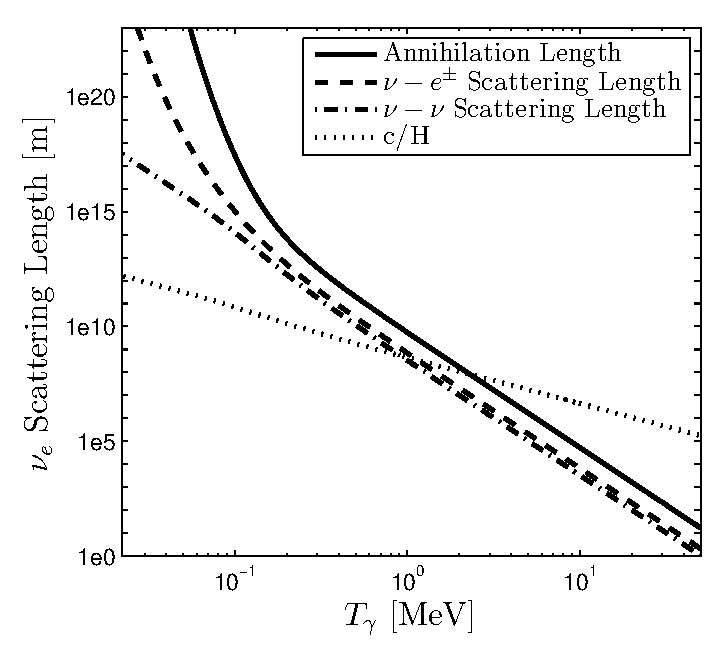
\includegraphics[height=6cm]{03-birrell/ParametricStudies/nu_e_scattering_length_eta_0_23.eps}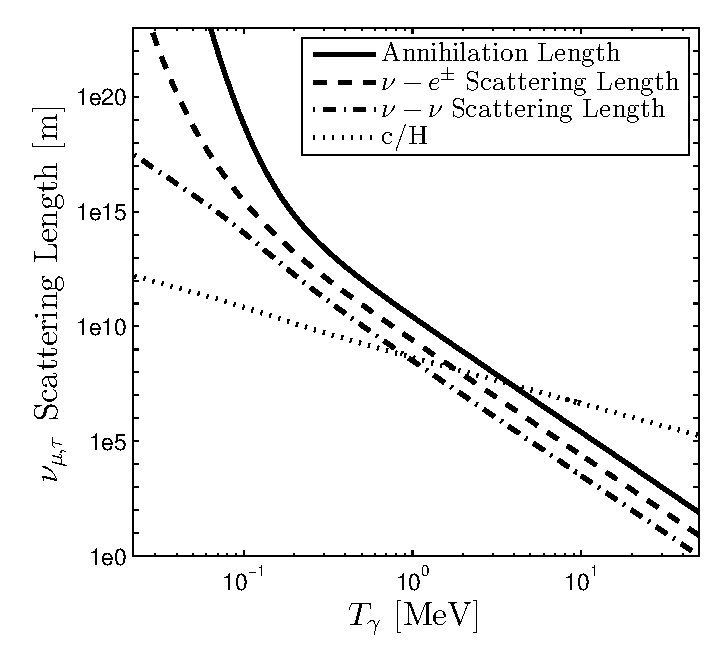
\includegraphics[height=6cm]{03-birrell/ParametricStudies/nu_mu_scattering_length_eta_0_23.eps}}
\caption{Comparison of Hubble parameter to neutrino scattering length for various types of processes for $\sin^2(\theta_W)=.23$. }\label{fig:scatt_length}
 \end{figure}
%%%%%%%%%%%%%%%%%%%%%%%%%%%%%%%%%%%%%%%


We now consider the the relaxation time for a given reaction, defined by $\tau=1/\Gamma$.  Suppose we have a time interval $t_f>t_i$  and corresponding temperature interval $T_f<T_i$ during which there is no reheating and the Universe is radiation dominated.  Normalizing time so $t=0$ corresponds to the temperature $T_i$ we have
\begin{equation}\label{ch6:H_eq}
\dot a/a=-\dot T/T,\hspace{2mm} H=\frac{C}{2Ct+T_i^2}\propto T^2
\end{equation}
where $C$ is a constant that depends on the energy density and the Planck mass.  Its precise form will not be significant for us.  Note that \req{ch6:H_eq} implies
\begin{equation}
1/H(t)-1/H(0)=2t.
\end{equation}

At $T\gg m_e$, the rates for reactions under consideration from tables \ref{table:nu_e_reac} and \ref{table:nu_mu_reac} scale as $\Gamma\propto T^5$.  Therefore, supposing $H(T_f)/\Gamma(T_f)=1$ (which occurs at $T_f=O(1\MeV)$ as seen in the above figures), at any time $t_f>t>t_i$ we find 
\begin{align}\label{relax_time}
\tau(t)/t=&\frac{2}{\Gamma(t)}\left(\frac{1}{H(t)}-\frac{1}{H(0)}\right)^{-1}=\frac{2T_f^5}{\Gamma(T_f)T^5}\left(\frac{T_f^2}{H(T_f)T^2}-\frac{T_f^2}{H(T_f)T_i^2}\right)^{-1}\\
=&\frac{2T_f^3}{T^3}\left(1-\frac{T^2}{T_i^2}\right)^{-1}.
\end{align}
Therefore, given any time $t_i<t_0<t_f$ we have
\begin{equation}\label{ch6:tau_eq}
\tau(t)<\tau(t_0)=\frac{2T_f^3}{T_0^3}\left(1-\frac{T_0^2}{T_i^2}\right)^{-1}\Delta t \text{ for all } t<t_0
\end{equation}
where $\Delta t=t_0-t_i=t_0$.

 The first reheating period that precedes neutrino freeze-out is the disappearance of muons and pions around $O(100\MeV)$, as seen in figure \ref{fig:energy_frac}, and so we let $T_i=100\MeV$. \req{ch6:tau_eq} is minimized at $T_0\approx 77.5\MeV$ at which point we have 
\begin{equation}
\tau(t)<10^{-5} \Delta t_0 \text{ for } t<t_0.
\end{equation}
This shows that the relaxation time during the period between $100\MeV$ and $77.5\MeV$ is at least five orders of magnitude smaller than the corresponding time interval.  Therefore the system has sufficient time to relax back to equilibrium after any potential non-equilibrium aspects developed during the reheating period.  Thus justifies our assumption that the neutrino distribution has the equilibrium Fermi Dirac form at $T=O(10 \MeV)$ when we begin our numerical simulation.

We demonstrate this numerically in figure \ref{fig:relax} where we have initialized the system at $T_\gamma=12\MeV$ with a non-equilibrium distriubtion of $\mu$ and $\tau$ neutrinos, giving them $\Upsilon=0.9$, and let them evolve.  We see that after approximately $10^{-3}$ seconds the system relaxes back to equilibrium, well before neutrino freeze-out near $t=1$s.

%%%%%%%%%%%%%%%%%%%%%%%%%%%%%%%%%%%%%%%
\begin{figure} 

\begin{minipage}{\linewidth}
\makebox[0.5\linewidth]%
{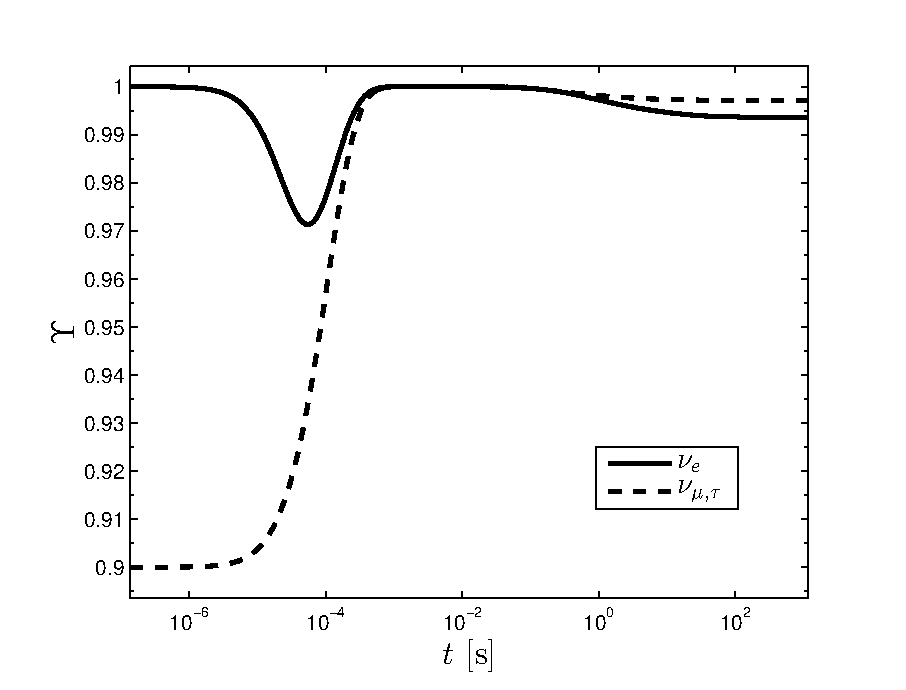
\includegraphics[height=6.2cm]{03-birrell/ScatteringIntegrals/Ups_relax.eps}}
\makebox[0.5\linewidth]%
{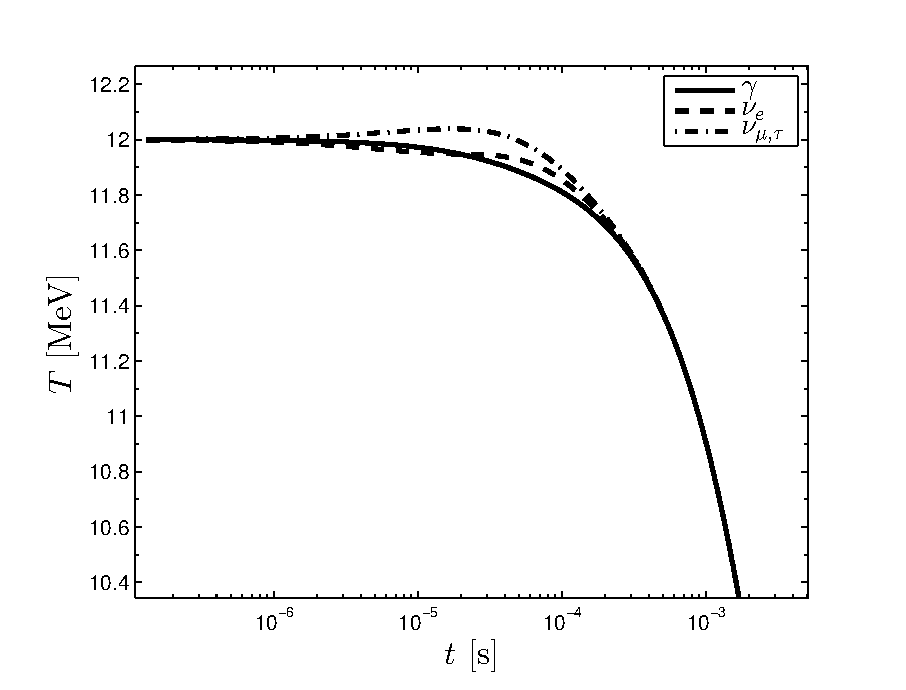
\includegraphics[height=6.2cm]{03-birrell/ScatteringIntegrals/T_relax.eps}}
\end{minipage}
\caption{Starting at $12\MeV$, this figure shows the relaxation of a non-equilibrium $\mu,\tau$-neutrino distribution towards equilibrium. The fugacities are shown in the left frame while the temperatures are shown in the right frame.\label{fig:relax}}
 \end{figure}
%%%%%%%%%%%%%%%%%%%%%%%%%%%%%%%%%%%%%%%



The attentive reader will notice that we have omitted here a discussion of flavor neutrino oscillations. If it weren't for the differences between the matrix elements for the interactions between $e^\pm$ and $\nu_e$ on one hand and $e^\pm$ and $\nu_\mu,\nu_\tau$ on the other, oscillations would have no effect on the flow of entropy into neutrinos and hence no effect on $N_\nu$, but these differences do lead to a modification of $N_\nu$.  In \cite{Mangano2005} the impact of oscillations on neutrino freeze-out for the present day measured values of $\theta_W$ and $\eta$ was investigated.  It was found  that while oscillations redistributed energy amongst the neutrino flavors, the impact on $N_\nu$ was negligible. We have neglected oscillations in our study and so, once the relevant neutrino properties are fully understood, the precision of the results could be improved by incorporating the effect of oscillations.




\subsection{Another Method for Computing Scattering Integrals}\label{app:dogov_method}
As a comparison and consistency check for our method of computing the scattering integrals, in this appendix we analytically reduce the collision integral down to $3$ dimensions by a method adapted from \cite{Dolgov_Hansen}.  The only difference between our treatment in this section and theirs being that they solved the Boltzmann equation numerically on a grid in momentum space and not via a spectral method.  Therefore we must take an inner product of the collision operator with a basis function and hence we are integrating over all particle momenta, whereas they integrate over all momenta except that of particle one.  For completeness we give a detailed discussion of their method.

 Writing the conservation of four-momentum enforcing delta function
\begin{equation}
\delta(\Delta p)=\frac{1}{(2\pi)^3}\delta(\Delta E)e^{i\vec z\cdot \Delta \vec p}d^3z,
\end{equation}
where the arrow denoted the spatial component, we can simplify the collision integral as follows
\begin{align}
R\equiv&\int G(E_1,E_2,E_3,E_4) S|\mathcal{M}|^2(s,t)(2\pi)^4\delta(\Delta p)\prod_{i=1}^4\frac{d^3p_i}{2(2\pi)^3 E_i}\\
=&\frac{1}{16(2\pi)^{11}}\int G(E_i) S|\mathcal{M}|^2(s,t)\delta(\Delta E)e^{i\vec z\cdot\Delta p}\prod_{i=1}^4\frac{d^3p_i}{ E_i}d^3z\\
=&\frac{2}{(2\pi)^{6}}\int G(E_i)K(E_i) \delta(\Delta E)\prod_{i=1}^4\frac{p_i}{E_i}dp_i z^2dz,\\
K=&\frac{p_1p_2p_3p_4}{(4\pi)^5}\int S|\mathcal{M}|^2(s,t)e^{i\vec z\cdot\Delta\vec p}\prod_{i=1}^4d\Omega_id\Omega_z.
\end{align}
We can change variables from $p_i$ to $E_i$ in the outer integrals and use the delta function to eliminate the integration over $E_4$ to obtain
\begin{align}
R=&\frac{2}{(2\pi)^{6}}\int1_{E_1+E_2-E_3>m_4}G(E_i)\left[\int_0^\infty K(z,E_i)z^2dz\right]dE_1dE_2dE_3,\\
p_i=&\sqrt{E_i^2-m_i^2},\hspace{2mm} E_4=E_1+E_2-E_3.
\end{align}
From tables \ref{table:nu_e_reac} and \ref{table:nu_mu_reac} we see that the matrix elements for weak scattering involving neutrinos are linear combinations of the terms
\begin{equation}
p_1\cdot p_2,\hspace{2mm} p_1\cdot p_3,\hspace{2mm}(p_1\cdot p_4)(p_2\cdot p_3), \hspace{2mm} (p_1\cdot p_2)(p_3\cdot p_4),\hspace{2mm} (p_1\cdot p_3)(p_2\cdot p_4).
\end{equation}
Therefore we must compute the angular integral term $K$ with $S|\mathcal{M}|^2$ replaced by elements from the following list
\begin{align}\label{matrix_element_pieces}
&1,\hspace{2mm}\vec p_1 \cdot\vec p_2,\hspace{2mm}\vec p_1 \cdot\vec p_3,\hspace{2mm}\vec p_1 \cdot\vec p_4 ,\hspace{2mm}\vec p_2\cdot\vec p_3,\hspace{2mm}\vec p_2\cdot\vec p_4 ,\hspace{2mm}\vec p_3\cdot\vec p_4 ,\\
& (\vec p_1 \cdot\vec p_2)(\vec p_3\cdot\vec p_4 ),\hspace{2mm}(\vec p_1 \cdot\vec p_4 )(\vec p_2\cdot\vec p_3),\hspace{2mm} (\vec p_1 \cdot\vec p_3)(\vec p_2\cdot\vec p_4 ),
\end{align}
producing $K_0$, $K_{12}$, $K_{13}$,...,$K_{1324}$.  All of these are rotationally invariant, and so we can always rotate coordinates so that $\vec z=z\hat z$.  This allows us to evaluate the $z$ angular integral
\begin{equation}
K=\frac{p_1p_2p_3p_4}{(4\pi)^4}\int S|\mathcal{M}|^2(s,t)e^{iz \hat z\cdot\Delta\vec p}\prod_{i=1}^4d\Omega_i.
\end{equation}

The remaining angular integrals are straightforward to evaluate analytically for each expression in \req{matrix_element_pieces}
\begin{align}
K_0&=\prod_{i=1}^4\frac{\sin(p_iz)}{z},\\
K_{12}&=-\frac{(\sin(p_1z)-p_1z\cos(p_1z))(\sin(p_2z)-p_2z\cos(p_2z))\sin(p_3z)\sin(p_4z)}{z^6},\\
K_{13}&=\frac{(\sin(p_1z)-p_1z\cos(p_1z))\sin(p_2z)(\sin(p_3z)-p_3z\cos(p_3z))\sin(p_4z)}{z^6},\\
K_{14}&=\frac{(\sin(p_1z)-p_1z\cos(p_1z))\sin(p_2z)\sin(p_3z)(\sin(p_4z)-p_4z\cos(p_4z))}{z^6},\\
K_{23}&=\frac{\sin(p_1z)(\sin(p_2z)-p_2z\cos(p_2z))(\sin(p_3z)-p_3z\cos(p_3z))\sin(p_4z)}{z^6},\\
K_{24}&=\frac{\sin(p_1z)(\sin(p_2z)-p_2z\cos(p_2z))\sin(p_3z)(\sin(p_4z)-p_4z\cos(p_4z))}{z^6},\\
K_{34}&=-\frac{\sin(p_1z)\sin(p_2z)(\sin(p_3z)-p_3z\cos(p_3z))(\sin(p_4z)-p_4z\cos(p_4z))}{z^6},\\
K_{1234}&=K_{1423}=K_{1324}=\prod_{i=1}^4\frac{(\sin(p_iz)-p_iz\cos(p_iz))}{z^2}.
\end{align}

To compute $\int_0^\infty K(z) z^2 dz$ we need to evaluate the following three integrals
\begin{align}
D_1=&\int_0^\infty \frac{\sin(p_1z)\sin(p_2z)\sin(p_3z)\sin(p_4z)}{z^2}dz,\\
D_2=&\int_0^\infty\frac{\sin(p_1z)\sin(p_2z)(\sin(p_3z)-p_3z\cos(p_3z))(\sin(p_4z)-p_4z\cos(p_4z))}{z^4}dz,\\
D_3=&\int_0^\infty\frac{\prod_{i=1}^4(\sin(p_iz)-p_iz\cos(p_iz))}{z^6}dz.
\end{align}
These expressions are symmetric under $1\leftrightarrow 2$ and $3\leftrightarrow 4$ and so without loss of generality we can assume $p_1\geq p_2$, $p_3\geq p_4$. We require $p_1\leq p_2+p_3+p_4$ (and cyclic permutations) by conservation of energy.  In the case where the above conditions all hold, we separate things into four additional cases in which the integrals can be evaluated analytically, as given in \cite{Dolgov_Hansen},\\
${\bf p_1+p_2>p_3+p_4\text{, \hspace{1mm} }p_1+p_4>p_2+p_3}${\bf :}
\begin{align}
D_1=&\frac{\pi}{8}(p_2+p_3+p_4-p_1),\\
D_2=&\frac{\pi}{48}((p_1-p_2)^3+2(p_3^3+p_4^3)-3(p_1-p_2)(p_3^2+p_4^2),\\
D_3=&\frac{\pi}{240}(p_1^5-p_2^5+5p_2^3(p_3^2+p_4^2)-5p_1^3(p_2^2+p_3^2+p_4^2)-(p_3+p_4)^3(p_3^2-3p_3p_4+p_4^2)\notag\\
&\hspace{7mm}+5p_2^2(p_3^3+p_4^3)+5p_1^2(p_2^3+p_3^3+p_4^3)).
\end{align}
${\bf p_1+p_2<p_3+p_4\text{, \hspace{1mm} }p_1+p_4>p_2+p_3}${\bf :}
\begin{align}
D_1=&\frac{\pi }{4}p_2,\\
D_2=&\frac{\pi }{24}p_2(3(p_3^2+p_4^2-p_1^2)-p_2^2),\\
D_3=&\frac{\pi}{120}p_2^3(5(p_1^2+p_3^2+p_4^2)-p_2^2).
\end{align}
${\bf p_1+p_2>p_3+p_4\text{, \hspace{1mm} }p_1+p_4<p_2+p_3}${\bf :}
\begin{align}
D_1=&\frac{\pi }{4}p_4,\\
D_2=&\frac{\pi}{12} p_4^3,\\
D_3=&\frac{\pi }{120}p_4^3(5(p_1^2+p_2^2+p_3^2)-p_4^2).
\end{align}
${\bf p_1+p_2<p_3+p_4\text{, \hspace{1mm} }p_1+p_4<p_2+p_3}${\bf :}
\begin{align}
D_1=&\frac{\pi}{8}(p_1+p_2+p_4-p_3),\\
D_2=&\frac{\pi}{48}(-(p_1+p_2)^3-2p_3^3+2p_4^3+3(p_1+p_2)(p_3^2+p_4^2)),\\
D_3=&\frac{\pi}{240}(p_3^5-p_4^5-(p_1+p_2)^3(p_1^2-3p_1p_2+p_2^2)+5(p_1^3+p_2^3)p_3^2-5(p_1^2+p_2^2)p_3^3\\
&\hspace{7mm}+5(p_1^3+p_2^3-p_3^3)p_4^2+5(p_1^2+p_2^2+p_3^2)p_4^3).\notag
\end{align}
We computed the remaining integrals numerically in several test cases for each of the reaction types in section \ref{nu_matrix_elements} and obtained agreement between this method and ours, up to the integration tolerance used.  However, the method we have developed in this chapter has the distinct advantage of resulting in a smooth integrand which then must be evaluated numerically.  The expressions obtained here are only piecewise smooth and therefore much costlier to integrate numerically.  In tests, the difference in integration time was found to be $1000$ times longer in some instances for the non-smooth integrand using an adaptive mesh integration method.  Since the cost of numerically solving the Boltzmann equation is dominated by the cost of computing the collision integrals, this is a very significant optimization.

\subsection{QED Corrections to Equation of State}\label{app:QED_corr}
At the time of neutrino freeze-out, the universe is at sufficiently high temperature for photons and $e^\pm$ to be in chemical and kinetic equilibrium.  The temperature is also sufficiently high for QED corrections to the photon and $e^\pm$ equation of state to be non-negligible.  We use the results given in \cite{Heckler:1994tv,Mangano2002} to include these in our computation by modifying the combined photon, $e^\pm$ equation of state
\begin{align}
P=P^0+P^{int},\hspace{2mm} \rho=-P+T\frac{dP}{dT}
\end{align}
where
\begin{align}
P^{int}=&-\frac{1}{2\pi^2}\int_0^\infty\left[\frac{k^2}{E_k}\frac{\delta m_e^2}{e^{E_k/T}+1}+\frac{k}{2}\frac{\delta m_\gamma^2}{e^{k/T}-1}\right]dk,\hspace{2mm} E_k=\sqrt{k^2+m_e^2}\\
\delta m_e^2=&\frac{2\pi\alpha^2}{3}+\frac{4\alpha}{\pi}\int_0^\infty \frac{k^2}{E_k}\frac{1}{e^{E_k/T}+1}dk,\hspace{2mm} \delta m_\gamma^2=\frac{8\alpha}{\pi}\int_0^\infty \frac{k^2}{E_k}\frac{1}{e^{E_k/T}+1}dk.
\end{align}
and $P^0$ is the pressure of a noninteracting gas of photons and $e^\pm$ in chemical equilibrium.



